\documentclass[sigconf]{acmart}
\usepackage[utf8]{inputenc}

\settopmatter{printacmref=false}
\renewcommand\footnotetextcopyrightpermission[1]{} % removes footnote with conference information in first column
\pagestyle{plain}

\usepackage{url}
\usepackage{hyperref}
\hypersetup{
    colorlinks=true,
    linkcolor=blue,
    filecolor=magenta,      
    urlcolor=cyan,
}
\urlstyle{same}


\usepackage{listings}
\usepackage{lipsum}
\usepackage{tabularx}
\usepackage{makecell}


% Enabling Javascript syntax highlight in code snippet - BEGIN 
% https://tex.stackexchange.com/questions/89574/language-option-supported-in-listings
\usepackage{color}
\definecolor{lightgray}{rgb}{.9,.9,.9}
\definecolor{darkgray}{rgb}{.4,.4,.4}
\definecolor{purple}{rgb}{0.65, 0.12, 0.82}
\definecolor{darkgreen}{rgb}{0, .64, 0}

\lstdefinelanguage{JavaScript}{
  keywords={typeof, new, true, false, catch, function, return, null, catch, switch, var, if, in, while, do, else, case, break},
  keywordstyle=\color{blue}\bfseries,
  ndkeywords={class, export, boolean, throw, implements, import, this},
  ndkeywordstyle=\color{darkgray}\bfseries,
  identifierstyle=\color{black},
  sensitive=false,
  comment=[l]{//},
  morecomment=[s]{/*}{*/},
  commentstyle=\color{purple}\^amily,
  stringstyle=\color{darkgreen}\ttfamily,
  morestring=[b]',
  morestring=[b]"
}

\lstset{
   extendedchars=true,
   basicstyle=\footnotesize\ttfamily,
   showstringspaces=false,
   showspaces=false,
   tabsize=2,
   breaklines=true,
   showtabs=false,
   captionpos=b,
   frame=single,
   xleftmargin=0.5em,
   belowcaptionskip=0em
}

\setlength{\belowcaptionskip}{-1em}
% Enabling Javascript syntax highlight in code snippet - END

\newcommand{\APIName}{Successorships }
\newcommand{\APINameNoSpace}{Successorships}

\newcommand{\APIshort}{Shippy }
\newcommand{\rpm}{\raisebox{.2ex}{$\scriptstyle\pm$}}

\newcommand{\accessed}{accessed 2017-12-11}

\usepackage{array}
\newcolumntype{L}[1]{>{\raggedright\let\newline\\\arraybackslash\hspace{0pt}}m{#1}}
\newcolumntype{C}[1]{>{\centering\let\newline\\\arraybackslash\hspace{0pt}}m{#1}}
\newcolumntype{R}[1]{>{\raggedleft\let\newline\\\arraybackslash\hspace{0pt}}m{#1}}


\graphicspath{{figures/}{pictures/}{images/}{./}}

%opening
\title{Zeroties: a Publish/Subscribe Service for Applications in Local Ad-Hoc Networks}

\author{Chris Satterfield \qquad Felix Grund}
\affiliation{
    \institution{University of British Columbia}
    \city{Vancouver} 
    \state{BC} 
  }

\begin{document}

\begin{abstract}

\end{abstract}

\maketitle

\section{Introduction}
\label{sec:introduction}

Throughout the last decade we have seen the Internet become the most commonly used infrastructure for communication. Regardless of physical location, people and their devices communicate via messengers and VoIP, and collaborate via live editing tools such as Google Docs, Sheets, and, Slides. 
At the same time, we have seen the paradigm of applications communicating over local area networks become increasingly common for certain scenarios like home entertainment (e.g. Google Chromecast, Apple Bonjour, Spotify Connect) or Wi-Fi printers. 
With the advancements of ``smart'' devices and the ``Internet of Things'' (IoT) it is likely that this trend will grow beyond these currently still narrowly scoped application domains.

The adoption of standards that eliminate the burden of manual configuration of network devices further contributes to this movement. One such standard that has received widespread usage is Zero-configuration networking~\cite{guttman_2001} and its protocols mDNS~\cite{cheshire_2013_mdns} for service advertisement and DNS-SD for service discovery~\cite{cheshire_2013_dnssd}.
Using the \textit{Zeroconf} protocols, devices can publish named services in the local network and discover such services automatically in an ad-hoc fashion.
While most applications for Zeroconf networks are shipped with specific hardware (e.g. Google Chromecast dongle) there have recently been attempts to provide software environments for developers to enable them write their own applications on already existing hardware infrastructure.
One such application was Mozilla FlyWeb\footnote{https://wiki.mozilla.org/FlyWeb}, an addon for the Firefox browser that made it possible to advertise and discover services from within Web applications through a JavaScript API.
In a previous project, we created \textit{Successorships}~\footnote{https://github.com/ataraxie/successorships}, a JavaScript library exposing an easy-to-use API to build fault-tolerant Zeroconf web applications.
Successorships was built on top of Mozilla Flyweb as one main part of its architecture.
This decision confronted us with significant problems:
\begin{itemize}
    \item FlyWeb had been declared abandoned by Mozilla even before we finished our work on our library.
    \item The implementation of the Zeroconf protocols in FlyWeb was slow to a degree that made our library fairly unusable in practice.
    \item FlyWeb contained a bug that made our library usable on MacOS only.
\end{itemize}

To overcome our troubles in Successorships, we introduce Zeroties (zero ties), a platform-independent asynchronous publish/subscribe service for Zeroconf advertisement and discovery.
We carefully reviewed different publish/subscribe designs~\cite{eugster_2003} and implemented a communication scheme based on \textit{asynchronous notifications}.
The operations exposed by Zeroties are as follows:
\begin{itemize}
    \item \textbf{Publish}: publish a Zeroties service and advertise it in the local network
    \item \textbf{Subscribe}: listen for updates on the list of available Zeroties services
\end{itemize}

Zeroties ships with two components: (1) a standalone OS-level daemon, and (2) addons for Chrome and Firefox that connect to this daemon.
With our addon implementations for Chrome and Firefox we aim to show that our approach translates well between different browsers and does not share the restrictions of FlyWeb.
Our browser addons expose an API to web applications that comprises the full service/discovery functionality of Zeroconf.
As a result, we have successfully eliminated the ties that prevented Successorships from usage in practice.

To evaluate Zeroties, we first created the webapp-based presentation for this project using Successorships in combination with the Zeroties daemon and the addon for Google Chrome.
Running the presentation on Chrome proved that we successfully broke ties with FlyWeb and Mozilla Firefox.
Furthermore, we could get a first sense in this example application that recovery from failures was significantly faster than with the previous version based on FlyWeb.
To evaluate these findings empirically, we analyzed the changes in performance with a test scenario based on the evaluation framework from Successorships.
We simulated nine failures on a small network of 6 nodes, first with the old FlyWeb-based implementation and then with the new version based on Zeroties.
While recovery took on average 12.93 seconds with FlyWeb, it took only 1.55 seconds using Zeroties, indicating a speedup of nearly a factor of 10.

In summary, we make the following contributions:
\begin{itemize}
    \item Zeroties, a asynchronous standalone publish/subscribe service for Zeroconf applications.
    \item Addons for Chrome and Firefox that make this service available to web applications.
    \item An empirical evaluation based on a Zeroties sample application indicating significant performance improvements.
\end{itemize}

The remainder of this paper is organized as follows: Section~\ref{sec:background_and_motivation} provides some background and motivation on why the idea for Zeroties came to be. Section~\ref{sec:approach} presents the system model and design goals of Zeroties, before Section~\ref{sec:implementation} describes its implementation. We evaluate Zeroties in Section~\ref{sec:evaluation} and suggest limitations and future work in Section~\ref{sec:limitations_and_future_work}. Section~\ref{sec:related_work} situates our work in the context of related research and Section~\ref{sec:conclusion} concludes the paper.




\section{Background and Motivation}
\label{sec:background_and_motivation}

We have been compelled by the idea to make the Zeroconf protocols available to web applications.
For example, consider the scenario of a group of people, each with their own device, collaborating on a Google Doc document.
Every keystroke in this document will need to be sent to a Google web server and then be ``pushed'' too all other group members.
Depending on geological location, this pattern of communication can impose roundtrips around the globe and lead to significant delays, despite the physical proximity of the devices.
The fact that not everybody around the globe is equipped with the newest network infrastructure makes this even more proplematic.

Zeroconf web applications provide a solution to this problem.
In the described Google Doc scenario, one person in the group would access the the Google Doc on the Internet and subsequently become a server in the local network.
Her device would then serve the resources it fetched from the actual web server to local clients who maintain a channel to this local server.
Effectively, only one Internet connection is required for the whole group, rather than one connection for every device\footnote{Obviously, this also has the advantage that only one device needs to have Internet connection in the first place. This is can be very interesting especially in scenarios where only dedicated participants in a network have such a connection, for example due to security restrictions.}, because all clients except the locally serving client access the original application (in this case Google Docs). Figure~\ref{fig:architecture_shift} illustrates this shift in architecture.

\begin{figure}[h]
    \centering
    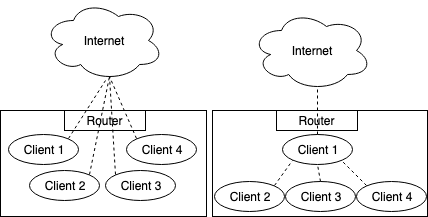
\includegraphics[width=\columnwidth]{architecture_shift}
    \caption{Architecture shift: on the left side is the traditional web application architecture where all devices are connected to a web server through the Internet. On the right is the Zeroconf architecture where only one client requires such a connection and becomes a server to all other clients in the network.}
    \label{fig:architecture_shift}
\end{figure}

Evidently, this pattern of communication has one major problem: it has a single point of failure, namely the client acting as a local server. 
Solving this problem was our motivation behind Successorships; whenever the currently serving client fails, a new client in the network is elected as the new server and connectivity in the network is re-established automatically.
Successorships provides a framework to build fault-tolerant Zeroconf web applications with an easy-to-use JavaScript API.
However, our decision to build it on Mozilla FlyWeb proved to be a major limitation.
Not only did we limit usage of our library to one specific browser vendor; we found out during the course of the project that Mozilla had already deprecated FlyWeb in favor of other priorities.
To make things worse, FlyWeb had a dependency to a Firefox core component (the module responsible for launching a web server within the browser) that was only shipped in a range of versions of the developer edition of Firefox.
In addition to this platform dependency that would, in essence, prevent our framework to be used in practice, the implementation of the Zeroconf protols in FlyWeb was incredibly slow.
According to our evaluation, recovery from failure of the currently serving client took more than 30 seconds in many cases.
With a continuously growing 'Limitations and Future Work' section, we were finally struck by the discovery of an unresolved issue in FlyWeb that made our framework only work on MacOS.
Despite our thoughtful and eager motivations, we had built a tool that nobody would ever use in practice.
Hence the call to get rid of this dependency entirely and provide our own layer below  Successorships.


\section{Approach}
\label{sec:approach}

\subsection{Environment and System Architecture}
\label{sub:architecture}

Figure~\ref{fig:architecture} illustrates the environment, placement of Zeroties, and the communication between components.
We describe the parts in the Figure by refering to the numbers in the ellipsis.

\begin{figure}[h]
    \centering
    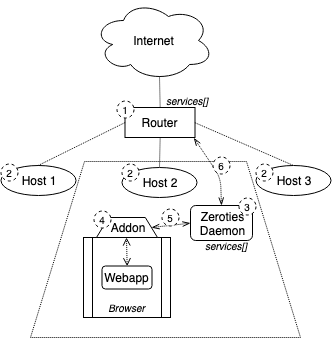
\includegraphics[keepaspectratio,width=6cm]{architecture}
    \caption{System architecture and environment in Zeroties.}
    \label{fig:architecture}
\end{figure}

\begin{enumerate}
\item \textbf{Router}~\footnote{Note that we use the term router somewhat casually in this context. Our notion of router is basically any part in the local network that serves the list of available Zeroconf services, as it can be obtained with DNS-SD. This may involve DHCP, IPv6 Router Advertisement Options or other mechanisms as specified on page 27f of~\cite{cheshire_2013_dnssd}. In other words, we simply call the component that stores the service list obtained from a DNS-SD-capable router.}: we use the protocols provided by Zeroconf (\cite{cheshire_2013_dnssd, cheshire_2013_mdns}) for Zeroties. 
In essence, this means that an authoritative list of currently available Zeroties services (as a subset of all Zeroconf services) can be obtained from the router at any given time.

\item \textbf{Hosts}: there can be an arbitrary number of hosts in our local network. A host can be any device in the network with an instance of Zeroties running (i.e. any device with an OS capable of Zeroconf/DNS-SD protocols).

\item \textbf{Zeroties Daemon}: the instance of Zeroties running on this device. 
This is an OS-level background application maintaining a list of services.
This list is a mirror of the service list obtained from the router by means of the Zeroconf protocols. 
The list of services constitutes the state of the distributed system\footnote{Note that there is a clear line between Successorships and Zeroties: Zeroties does not know about the arbitrarily complex state of Successorships or any other app that builds on Zeroties.}.
We originally intended to integrate this application into browser addons, but were restricted by browser policies.
In particular, there is no possibility to start a web server or publish a Zeroconf service from within a browser addon.
Hence our alternative solution of an OS-level app that communicates with our browser addons through stable bi-directional message channels.

\item \textbf{Browser Addons}: we require browser addons that mediate between web applications and the Zeroties daemon. These addons expose a JavaScript API to apps built on top of Zeroties.
We have implemented addons for Google Chrome and Mozilla Firefox that constitute such a mediator and we have run Successorships apps with these addons (see Section~\ref{sec:evaluation}).
These addons use Zeroties as a publish/subscribe service.
Furthermore, we have built a UI in form of a browser menu button and a popup that shows the currently available list of services.
This UI is refreshed on-the-fly and mirrors the list of services in Zeroties.
Note that the Zeroties daemon itself is not restricted to these addons; they are only required for web applications running in browsers.
Different applications can utilize the services provided by the Zeroties daemon without these components.

\item \textbf{Publish/Subscribe operations}: applications built on top of Zeroties interact with the Zeroties daemon using the common publish/subscribe operations.
\textit{Publish} is the publishing of a Zeroties service and \textit{subscribe} makes the application receive changes to the list of available Zeroties services. 

\item \textbf{Advertisements and service discovery}: the Zeroties daemon maintains a list of Zeroties services that is obtained from the router.
In a sense, Zeroties acts as a middleware between the router and applications built on top of Zeroties (applications using Successorships as framework being one example). 
Whenever a Zeroties application publishes a service using the Zeroties publish/subscribe API, this will result in the publishing of a service in the network (service advertisement). 
The second part of this communication channel is service discovery.
We describe both service advertisement and service discovery in more detail in Section~\ref{sec:implementation}.
\end{enumerate}


\subsection{Design Decisions and Goals}
\label{sub:design}

Zeroties is based on system models as in the example described in Section~\ref{sec:background_and_motivation}: local ad-hoc network applications. We claim that there is a dedicated set of such applications, for example:
\begin{itemize}
\item a project presentation at a meetup where the audience can connect to the presentation and interact with it.
\item an application for printer control in an office.
\item an application for the heating system of a hotel.
\item multiplayer mode for browser-based games.
\end{itemize}

Such applications have in common a limited number of nodes (generally < 100) and comparably lax requirements for time-to-recovery from system failures: certain downtimes can be tolerated as long as a consistent state is reached eventually.
For example, a running application converging to a consistent state within a time frame of multiple seconds after failures is acceptable.
Our particular goals behind Zeroties are described in the following paragraphs.

\textbf{Publish/subscribe strategy}. 
We reviewed the different publish/subscribe strategies described in~\cite{eugster_2003} and decided to focus on an asynchronous invocation/callback style communication pattern as described in~\cite{eugster_2003}§3.3. 
Asynchrony is essential for the communication between the Zeroties daemon and its applications.
For example, applications built on Zeroties should not be blocked while waiting for the successful advertisement of a service, but rather perform this action in the background while the application remains responsive in the foreground.

\textbf{Consistency guarantees}.
The shared state in Zeroties systems is defined by (1) the list of currently available Zeroties services, and (2) the application-defined state that is shared between hosts in the network.
If an instance is not up-to-date with this state, this can have different consequences. 
First, as long as applications are not notified that a new service has been created, that service remains unavailable.
Second, a service that has failed but remains in the list can result in an error upon connecting to that service. 
Third, if notifications about updates of the application-defined state are delayed between hosts, this can have significant consequences.
However, given our described system model of local ad-hoc network applications, we postulate that it is sufficient for most use cases if hosts converge to a consistent state \textit{eventually} and therefore decided for \textit{optimistic replication}~\cite{saito_2005}.
The paper defines \textit{eventual consistency} as ``a weak guarantee [that] is enough for many optimistic replication applications, but some systems provide stronger guarantees, e.g., that a replica's state is never more than one hour old''.
Due to our requirements for an asynchronous publish/subscribe pattern and our awarenes that, according to the CAP theorem~\cite{gilbert_2012} we cannot achieve both high consistency and availability, our work can be considered as trading consistency in favor of high availability.
Nevertheless, we consider the time frames for reaching consensus in our previous project (> 30 seconds in many cases) as insufficient and we want our new system to do so within a time frame of \textit{5 seconds}.

\textbf{Fault tolerance}:
In the case of Zeroties, fault tolerance is directly connected to consistency guarantees.
Take Successorships as an example for a Zeroties application and assume the scenario of a failing server~\footnote{In the Successorships example, by \textit{server} we refer to the \textit{the currently serving client}. Remember that in our world any client of the web application can become a server.}.
The service that was offered by the failed server will be removed from the list of available Zeroties services and the change will be propagated to Zeroties applications that poll information from the router (see Section~\ref{sub:architecture}).
The application can then decide how to deal with this change.
In the Successorships example, this will involve the selection of a new server (and therefore a new Zeroties service) and other clients connecting to it.
In that sense, the system will have recovered from the failure of the server (and therefore have converged to a consistent state), as soon as (1) the failed service was removed from the list, (2) the newly elected service was added to the list, and (3) all changes propagated to all clients in the system.
Consequently, Zeroties enables its applications to recover from failures in the same time frame as the system reaches consensus.

\textbf{Performance}:
As described earlier, the performance of our previous implementation of Zeroconf based on FlyWeb showed significant bottlenecks and proved insufficient for practical usage.
With Zeroties we had a few concrete goals in mind regarding time frames. 
First, the \textit{publishing of services} and \textit{notifications about new services} from the perspective of a Zeroties application should take \textit{less than 5 seconds}.
\textit{Communication between Zeroties and its applications} should be in the range of \textit{milliseconds}.

\textbf{Reliability}:
Our system should remain highly reliable as long as our DNS-SD communication scheme between Zeroties and the router is robust and the communication channels between Zeroties and its applications are stable.

\textbf{Polling strategy:}
We decided for a polling strategy for obtaining the list of services from the network router using DNS-SD.
The list of available services is updated based on changes detected between the last version of the services list in the Zeroties daemon and the most recently polled services list.
Clearly, this polling strategy will impose traffic on the local network, with all Zeroties hosts polling the router for the services list.
However, we argue that frequent changes in the available services list and the presumed low number of nodes in our system model justifies this approach.
A different strategy which could allow for a larger number of nodes without the potential problem of overloading the router with requests would be to implement this communication with a dedicated Zeroties leader and followers, for example using Paxos~\cite{lamport_2001} or Raft~\cite{ongaro_2014}.
However, this would mostly be a transformation of communication between Zeroties hosts and the router towards communication between Zeroties hosts. 
More importantly, we would waive the advantage of the direct use of the authoritative list of services maintained by the network.
Nevertheless, we are aware that a design with the leader-and-followers approach, despite adding significant complexity, would have advantages as soon as Zeroties networks reach a certain size.




\section{Implementation}
\label{sec:implementation}

This section describes the languages and platforms on which Zeroties is based.
It then illustrates the different components in Zeroties: the daemon, the browser addon, and the communication between these components.

\subsection{Languages and Platforms}
\label{sub:languages_and_platforms}

All components are written in JavaScript. 
The Zeroties daemon is written using Node.js\footnote{https://nodejs.org/en/, accessed 2019-04-17}, the browser addons are written with the vendor-specific addon frameworks.
We decided on JavaScript for all components due to several reasons:
\begin{itemize}
\item We wanted the OS-level Zeroties daemon to be as platform-independent as possible. 
Node.js is a stable environment on all major operating systems by now.
\item We wanted to lean on a library implementing the low-level Zeroconf protocols.
We found a capable, mature, and well-maintained library, \textit{dnssd}\footnote{https://www.npmjs.com/package/dnssd, accessed 2019-04-17} available for this purpose on Node.js.
\item Browser addons must be implemented in JavaScript.
Despite the fact that we could not integrate the core Zeroties functionality into our browser addons (see Section~\ref{sec:approach}) we still wanted to avoid  introducing a language barrier that would prevent us to do so even without browser-specific restrictions.
\item Starting a HTTP server and a WebSocket server in Node.js and connecting to these servers from an addon is inherently straight-forward.
This functionality was required for our purpose.
\end{itemize}

\subsection{Zeroties Daemon}
\label{sub:zeroties_daemon}

At the core of Zeroties is the Zeroties daemon.
This is the piece of software that any application wishing to make use of the Zeroties services must connect to.
The daemon runs continuously in the background on the user's operating system with a server to handle interactions with Zeroties applications.
Zeroties applications are provided the following two pieces of core functionality by interacting with the Zeroties daemon:
\begin{itemize}
    \item The ability to publish services on the local network, via mDNS.
    \item Notifications when the list of services available on the local network changes, as discovered via DNSSD.
\end{itemize}
The Zeroties daemon is also responsible for handling any client HTTP request or WebSocket connection to the server published by a Zeroties application.
Instead of handling these events directly, the daemon acts as a proxy, forwarding the events to the Zeroties app as approriate.
This allows developers of Zeroties applications to easily define custom routing for HTTP requests recieved, and define custom actions to handle different WebSocket events.

All communication between Zeroties applications and the Zeroties daemon is made via a WebSocket connection, following the protocol outlined as follows: on connecting to the daemon, applications are automatically subscribed to recieve notifications about changes to the list of available Zeroties services.
The daemon repeatedly polls the network to retrieve the current list of Zeroties services using the DNSSD protocol.
If the list of services retrieved from the network differs from the one currently held by the daemon, an event is triggered.
This event is fired over the WebSocket connection to all listening Zeroties applications.
To publish a service, a Zeroties application sends a message to the daemon containing the name of the service to publish.
The Zeroties daemon then spins up an HTTP server and a WebSocket server listening on the same port, and advertises the newly available service over the local network via mDNS.


% what it is:
% - the core Zeroties daemon
% - any application wishing to use Zeroties must communicate with this app

% what does it do:
% - facilitates publishing services on the local network
% - notifies clients on updates to available services list
% - handles client connections and forwards requests/messages to Zeroties app for handling (acts as a proxy)


% how does it work:
% - services list is maintained/updated via mdns/dnssd
% - Zeroties apps connect to the Zeroties daemon via a Websocket connection
% - on connecting, clients are automatically subscribed to recieve updates about changes to the list of services
% - Zeroties apps notify the Zeroties daemon if they wish to publish a server
% - clients connect to Zeroties daemon server
% - server forwards to Zeroties app for handling via websockets
% - Websocket communication allows us to define http request handling behaviour in the browser
% - request/response protocol

% could it be improved?:


\textbf{Zeroties Communication Protocol.} Communication with the Zeroties daemon must follow a certain protocol.

\begin{itemize}
\item \textit{Messages to the Zeroties Daemon}: at the moment, there is only one supported message that may be sent to the Zeroties Daemon unprompted: the \texttt{publish} message.
The message must send a JSON string of the following format: 
\begin{lstlisting}[breaklines]
{method: "publish", payload: {name: appName}}
\end{lstlisting}
This is the message that informs the Zeroties daemon that the application wishes to publish a service.
\item \textit{Messages from the Zeroties Daemon}: any app connected to the Zeroties daemon should expect to receive and handle a message in the following format:
\begin{lstlisting}[breaklines]
{method: "servicesChanged", services: <array of services>}
\end{lstlisting}
This is the message sent by the Zeroties daemon whenever a change in the list of Zeroties services is detected.
Table~\ref{tab:zeroties_protocol} outlines the messages sent from the Zeroties daemon sent to its applications that publish a service, as well as the expected responses to these messages.
\end{itemize}


\begin{table*}[h]
\small
\centering
\caption{The messages sent to Zeroties apps by the Zeroties daemon, and the responses which are expected back. After recieving a \texttt{wsForwardResponse}, the daemon will respond again with a \texttt{wsProxyHandshake} message.}
\def\arraystretch{2}
\begin{tabularx}{\textwidth}{l|l|l|l}
\textbf{Method} & \textbf{Response} & \textbf{Response to response} & \textbf{\pbox{9.5cm}{Purpose}}\\
\hline
\texttt{request} & \texttt{response} & & \pbox{9.5cm}{Dispatches an incoming HTTP request to the Zeroties App for handling. Waits for a response containing the serialized response}\\ \hline
\texttt{wsForward} & \texttt{wsForwardResponse} & \texttt{wsProxyHandshake} & \pbox{9.5cm}{Notifies the Zeroties app of an incoming WebSocket connection and establishes a proxy connection}\\ \hline
\texttt{wsForward} & \texttt{init} & & \pbox{9.5cm}{To complete the proxy connection, the Zeroties app must send an init message over the proxy connection once it is open}\\
\end{tabularx}
\label{tab:zeroties_protocol}
\end{table*}

\subsection{Browser Addons}
\label{sub:browser_addons}

The Zeroties browser addon is an intermediary layer that easily allows web applications to function as Zeroties apps.
They expose a simple API that abstracts away the underlying complexities of proxy communication with the Zeroties server.
The addon works by injecting the API script into all accessed webpages using a content script.

\textbf{API for web applications.}
The Zeroties addon API consists of two functions:
\begin{itemize}
\item \texttt{navigator.publishServer(appName)} sends a message to the Zeroties daemon, which then attempts to publish a server with the specified name.
It returns a Promise, which resolves to a server object. 
From this server object, behaviour for handling HTTP requests and WebSockets can be defined.
\item \texttt{window.addEventListener("zerotiesServicesChanged", callback)} listens for the  \texttt{zerotiesServicesChanged} event. This event is triggered by the Zeroties daemon whenever the list of Zeroties services available has changed.
The second parameter is a callback function which recieves the updated services list as its argument.
\end{itemize}

This API roughly mimicks the one that was provided by FlyWeb, so migrating a (Successorships-)FlyWeb application to Zeroties involves only minimal changes\footnote{Obviously, we did not want to keep the name \texttt{flywebServicesChanged} for our event.}.

The Zeroties addon also contains a browser menu button that renders a popup upon click showing a list of currently available services.
This list is updated live through the WebSocket channel to the Zeroties daemon.
Figure~\ref{fig:addon} shows a screenshot of this popup with a single service being published.
A click on a service in this list will open a new tab and connect to the service as a client.

\begin{figure}[h]
    \centering
    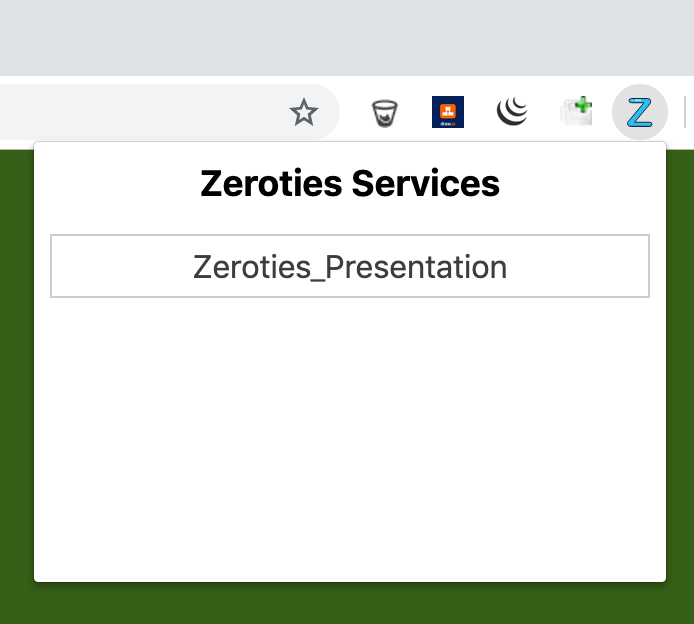
\includegraphics[keepaspectratio,width=6cm]{addon}
    \caption{Addon services menu.}
    \label{fig:addon}
\end{figure}

% what is it:
% - addons for chrome and firefox
% - an example of a Zeroties app

% what does it do:
% - provides a simple interface to webapps for communcation with the Zeroties daemon
% - abstracts away all the websocket nonsense
% - popup shows all published zeroties services on the local network

% how does it work:
% - communicates with the Zeroties daemon via websockets following request/response protocol
% - injects a script to webapps which exposes the api via window/navigator

\subsection{Communication and Control Flow in Zeroties}
\label{sub:communication}

This section discusses the flow of control and the communication between Zeroties apps and the Zeroties daemon, using Successorships as an example.
Listing~\ref{lst:publish_service} shows an example usage of the \texttt{publishServer} API.
The functions \texttt{onFetch}, \texttt{onWebsocket}, and \texttt{onClose} are event listeners that are called when their respective events are dispatched.

\begin{lstlisting}[caption={Publishing of a service},label={lst:publish_service}]
navigator.publishServer(Shippy.internal.appName()).then(function(server) {
  // ...
  server.onfetch = onFetch;
  server.onwebsocket = onWebsocket;
  server.onclose = onClose;
  // ...
}).catch(function (err) {
  // ...
});
\end{lstlisting}

When the \texttt{onWebsocket} function is called, a WebSocket connection with the Zeroties daemon is established.
This WebSocket serves as the main channel of communication between the daemon and the addon, which interacts directly with the web application.
Whenever a client triggers an event on the published server, for example upon recieving an HTTP request, it is forwarded to the addon via a WebSocket message.
In the case of an HTTP request, the \texttt{onFetch} function is called, which generates a response to the request.
The response is then serialized and sent back over the WebSocket as the payload of another message.
Finally, the response is deserialized by the Zeroties daemon and dispatched back to the appropriate client.
To make sure responses are sent back to the correct client, all messages in this series of events are accompanied by a unique identifier that is generated when the HTTP request is first recieved.

WebSocket connection events follow a similar control pattern.
When the published server recives a WebSocket connection, the Zeroties daemon notifies the addon of the new connection with a WebSocket message.
The addon then creates a new WebSocket connection with the daemon. 
This means that for each client connected to the server, there is a proxy WebSocket between the daemon and the addon.
This facilitates pseudo-direct communication between the server webapp and its clients.
WebSocket messages are sent from the client to the published server, and then forwarded by the daemon over the proxy connection to the server webapp.
The reverse is true for messages sent from the server webapp to the client.

Listing~\ref{lst:service_discovery} shows an example of subscribing to changes in the Zeroties services list.
This is a fairly straightforward process: the Zeroties daemon polls the network for changes in the services list using DNSSD.

\begin{lstlisting}[caption={Service discovery},label={lst:service_discovery}]
window.addEventListener('zerotiesServicesChanged', function (event) {
  // ...
});
\end{lstlisting}

When a change is detected, the daemon sends a message over the WebSocket connection to the addon.
This message contains the updated services list.
The addon then dispatches a \texttt{zerotiesServicesChanged} event on the global \texttt{window} object with the updated services list as payload.


\section{Evaluation}
\label{sec:evaluation}

\subsection{Sample Successorships Application}

In our previous project, we created a web application using the presentation framework \textit{Reveal.js}~\footnote{https://github.com/hakimel/reveal.js/, accessed 2019-04-17} to present Successorships to graduate students of the computer science department of the University of British Columbia.
The application used the Successorships API that made use of the Zeroconf protocols based on FlyWeb.
Obviously, the presenters had to have a Mac computer and a dedicated old version of Firefox Developer Edition with the FlyWeb addon installed to be able to present.
Moreover, the previously mentioned performance problems were clearly visible, with recovery of the system from intentionally injected faults taking over 20 seconds at times.
In a similar fashion, we presented Zeroties to an audience of graduate students at the same university.
The presentation technicalities remained the same, except that the API usage within Successorships was changed from FlyWeb to Zeroties.
To demonstrate this new independence of Firefox, the presentation was performed on Google Chrome.
A significant decrease in time-to-recovery after failure could clearly be observed with the system recovering in very few seconds.

\subsection{Empirical Evaluation}

We reproduced the performance measurements from the previous paper in order to analyze changes in performance from the old to the new version of Successorships.
We collected traces for system recovery for the following scenario, first with the old FlyWeb-based version on Mozilla Firefox, and then with the new Zeroties-based version on Google Chrome:
\begin{itemize}
\item One node starts the app and becomes the server.
\item 5 nodes start the app and become clients.
\item The server broadcasts 7 messages to all clients.
\item The server dies and the next successor becomes the server.
\item The other 4 clients become clients to the new server.
\end{itemize}

This process was first repeated until only the last node remained and became the server.
Afterwards, 5 more nodes started the application and became clients of that last remaining node from the last run that was now serving.
The process was then repeated once more until the last node was finally terminated.
In total, this process therefore involved 9 recoveries from server failures.
The scenario was performed on one machine where one node constituted one browser window.
While we acknowledge that a multi-machine experiment would have been more representative, we argue that for the analysis of performance changes between the two version this infrastructural change would not be significant.

Table~\ref{tbl:eval:time-to-recovery} shows the time to recovery in seconds for the described scenario with FlyWeb and Zeroties.
It is visible, that the Zeroties version recovered from failures nearly 10 times faster with little variation.
Figure~\ref{fig:eval:server-recovery} compares the cumulative distribution between the two versions that confirms this finding.

\begin{table}
    \caption{Time-to-recovery in seconds with FlyWeb and Zeroties}
    \label{tbl:eval:time-to-recovery}
    \centering
    \begin{small}
    \begin{tabular}{C{1cm}|C{2.5cm}|C{2.5cm}}
    \hline
    \bfseries Failure \# & \bfseries FlyWeb & \bfseries Zeroties \\
    \hline
1 & 15.554 & 1.817 \\
2 & 15.05 & 1.607 \\
3 & 13.183 & 1.701 \\
4 & 13.07 & 1.659 \\
5 & 14.836 & 1.795 \\
6 & 10.652 & 1.726 \\
7 & 11.32 & 1.244 \\
8 & 11.212 & 1.138 \\
9 & 11.473 & 1.269 \\
    \hline
    \end{tabular}
    \end{small}
\end{table}

\begin{figure}[h]
    \centering
    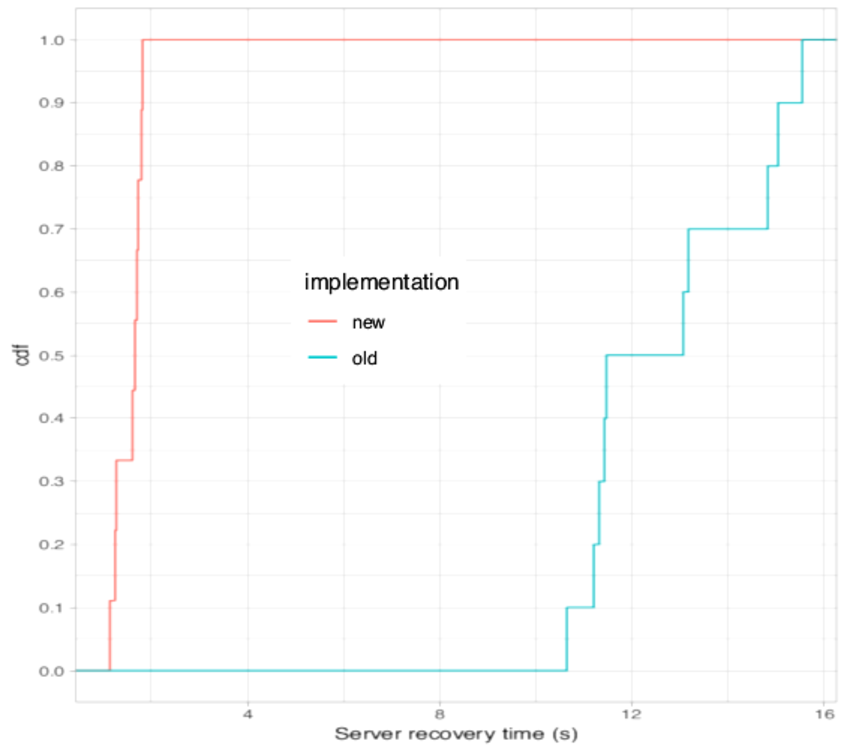
\includegraphics[keepaspectratio,width=\columnwidth]{server-recovery}
    \caption{Comparison of CDFs for server discovery between FlyWeb-based and Zeroties-based versions of Successorships.}
    \label{fig:eval:server-recovery}
\end{figure}

\section{Limitations and Future Work}
\label{sec:limitations_and_future_work}


\section{Related Work}
\label{sec:related_work}

\textbf{Zeroconf.}
Several researchers have investigated Zeroconf~\cite{Gunes2002, Bohnenkamp2003, Jara:2012:IPv6DNS-SD}.
For instance, \cite{hong2007accelerating} discusses that Zeroconf service discovery may cause overhead to the network while discovering new services.
Thus, they propose an algorithm to accelerate service discovery based on network topology changes.
Since a server failure would imply a change in the network topology, i.e. the server node being removed from the topology, 
client nodes in our implementation could use their approach to accelerate service discovery. 
Nonetheless, their implementation uses Linux Wireless extensions, which may not be accessible within a browser.
Thus, we used the FlyWeb service discovery implementation.

In~\cite{stolikj2016context}, Stolikj et al. argue that the number of published services in a network may also slow down service discovery.
As a solution, they propose a context-based approach, where queries specify which services they are interested in.
This approach is highly suitable for our work and we could use it to filter \APIshort services.
However, their approach changes service discovery queries and we question whether this could be easily integrated with existing devices.


\textbf{Local Networking APIs.}
Published in 2008, Universal Plug and Play (UPnP) is another widely-deployed set of networking protocols that facilitate discovery and interaction between devices on the same network, with minimal configuration.
Since it leverages common protocols (HTTP/XML/SOAP on UDP/IP) and is agnostic to the link medium, it is truly cross-platform, extending not only to phones and laptops but also to printers, WiFi routers, and audio-visual equipment, to name a few examples.
UPnP has been characterized as consisting of protocols that are more specific to particular classes of devices and applications; this is in contradistinction to Zeroconf, which aims to provide a device-agnostic foundation on which any device class or application-level protocol can build.~\footnote{\url{http://www.zeroconf.org/zeroconfandupnp.html}}

More recently in 2017, as part of its \textit{Nearby} project, \textit{Google} released its \textit{Connections} API, which enables Android devices in close proximity to one another to communicate in a peer-to-peer fashion.~\footnote{\url{https://developers.google.com/nearby/connections/overview}, accessed 2017-12-11}
This is done over a seamless mix of Bluetooth and WiFi hotspots.
Unfortunately, Google has only made this API available on the Android platform; we seek a solution that is truly cross-platform.

\textbf{In-browser web servers.}
An early example of fully in-browser web server technology was \textit{Opera Unite} (2009)\footnote{\url{http://help.opera.com/Windows/12.10/en/unite.html, accessed 2017-12-11}}.
This extension to the Opera browser enabled users to serve general-purpose Web applications directly from their browsers. 
Communication between clients and servers in this way could either be via Opera Unite's proxy servers, which also offered a name registering and directory service, or direct peer-to-peer, the latter requiring more advanced technical configuration.
Importantly, Opera Unite applications were constrained to be written as Opera ``Widgets''\footnote{An Opera Widget is an application that runs on Opera's now-deprecated Widget Engine, which allows such apps to be run independently of the browser.}.
Though the service was popular with a sizeable subset of Opera users, especially for purposes such as file sharing and media streaming, Opera eventually retired Unite in 2012 to consolidate the multiple extension frameworks offered in its browser.\footnote{http://www.instantfundas.com/2012/04/opera-to-discontinue-unite-widgets-and.html}

% TODO (PTC): Possibly add some notes on Web Server Chrome, and PeerServer.

\section{Conclusion}
\label{sec:conclusion}


\bibliographystyle{abbrv}
\bibliography{paper}

\end{document}

